\subsection{Réseaux}
\label{subsection:res}

Dans les sections \ref{subsubsection:fonctionnement_reseau} et \ref{subsection:network_implementaion}, nous avons présenté l'oganisation et l'implémenation du réseau de communications de Simterpose. Nous souhaitons maintenant évaluer les performances de notre implémenration à travers divers tests.

\subsubsection{Protocole}
L'objectif principal étant de montrer qu'il est possible de faire de la virtualisation légère, nous souhaitons d'abord mesurer l'\textit{overhead} dû à l'utilisation de Simterpose. De cette façon, si le surcoût d'utilisation de notre émulateur est négligeable on pourra conclure que ce type de virtualisation est possible pour le réseau. Dans un second temps, nous souhaitons mesurer les performances des deux types de médiations que nous avons implémentés. Cela nous permettrait de savoir le type de médiation qu'il vaut mieux utiliser selon l'application que l'on souhaite exécuter.

Pour effectuer nos expériences, nous avons choisi deux applications réseau d'échanges de messages. La première application consiste à faire communiquer un client et un serveur en envoyant au serveur un million de messages de petite taille. La seconde va envoyer depuis un client un message de 1Mo à un serveur. Le protocole pour chaque expérience a été d'exécuter 20 fois chaque application en utilisant les mêmes appels systèmes pour communiquer les messages (\texttt{sendto}/\texttt{recvfrom} et \texttt{sendmsg}/\texttt{recvmsg}), puis une moyenne du temps d'exécution ainsi qu'une mesure des temps minimum et maximum ont été conservées.

\subsubsection{Overhead conçernant le temps d'exécution}
Afin de mesurer l'\textit{overhead} produit par Simterpose, notre expérience consiste à exécuter les deux applications réseaux choisies sur une machine en utilisant uniquement le réseau local puis en utilisant Simterpose en suivant le protocole présenté plus haut. Ainsi, en comparant les temps d'exécution des applications sur les deux types d'architecture nous pourrons calculer l'\textit{overhead}. Les résultats de ces expériences sont présentés Figures \ref{Network_Big_Local} et \ref{Network_Little_Local}.

Dans le cas de l'envoi de plusieurs petits messages le temps moyen d'exécution en local est d'environ 3 secondes, avec Simterpose on arrive à 72 secondes en \textit{full mediation} et à 75 secondes en \textit{médiation par traduction d'adresse}. On a donc une exécution qui prend 25 fois plus de temps. De même, lors de l'envoi d'un gros message le système met 0,01 secondes en moyenne pour exécuter l'application alors que Simterpose met entre 1 et 1,1 secondes selon le type de médiation. Cette exécution prendra donc 100 fois plus de temps si on souhaite réellement mettre en place notre émulateur.

\begin{figure}
  \centering
    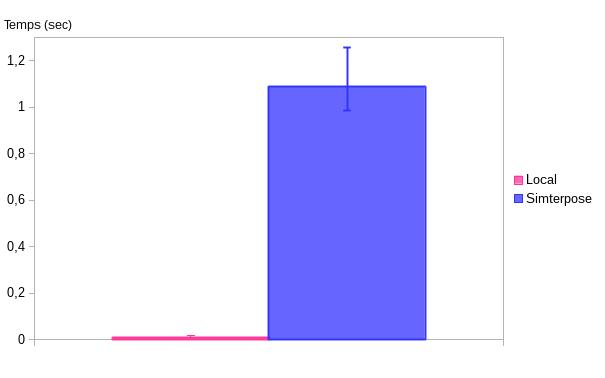
\includegraphics[scale=0.5]{mesures/graph/Bigmsg_local.jpg}
    \caption{Temps d'exécution lors de l'envoi d'un message de 1Mo avec et sans Simterpose.}
    \label{Network_Big_Local}
\end{figure}

\begin{figure}
  \centering
    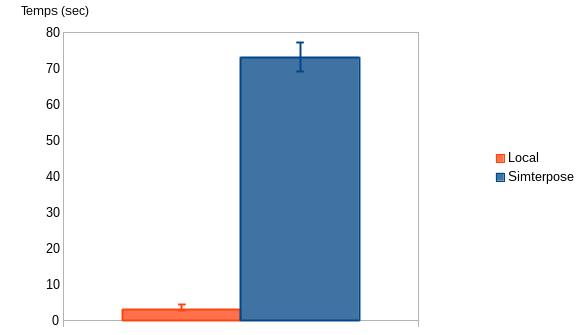
\includegraphics[scale=0.5]{mesures/graph/Littlemsg_local.jpg}
    \caption{Temps d'exécution lors de l'envoi d'un million de messages de 128o avec et sans Simterpose.}
    \label{Network_Little_Local}
\end{figure}
  
Néanmoins, cet écart s'explique par les nombreux appels systèmes et changements de contexte que nécessite Simterpose de par son utilisation coûteuse de \texttt{ptrace} en plus de l'exécution de l'appel système lui-même lorsqu'on utilise \textit{médiation par traduction d'adresse}. Pour la première expérience on peut considérer que cet \textit{overhead} représente un cas extrême car les utilisateurs en général ne testent pas leurs applications en envoyant des millions de message entre un client et un serveur. De plus, du point de vue humain une exécution de 1ms ou 1s dans le second cas ne change pas grand chose pour notre perception. Ainsi, on peut considérer que l'\textit{overhead} produit par Simterpose sur le temps d'exécution est acceptable.

\subsubsection{Quelle médiation pour quel type d'application}
 Cette seconde expérience vise à comparer les deux médiations que nous avons implémentés. Pour cela, en suivant le protocole présenté plus haut on va exécuter les deux applications réseau choisi en utilisant les deux types de médiations. Les résultats de notre expérience sont présentés Figures \ref{Network_Big_Mediation} et \ref{Network_Little_Mediation}.

 \begin{figure}[H]
  \centering
    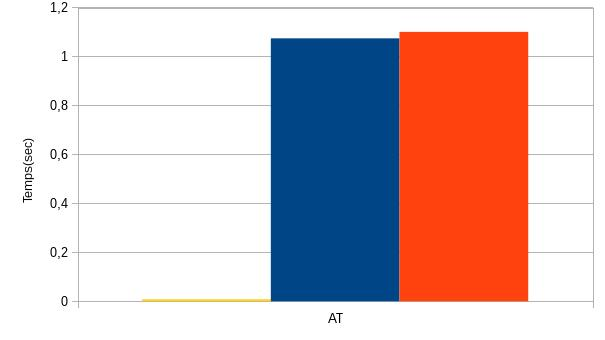
\includegraphics[scale=0.5]{mesures/graph/Bigmsg.jpg}
    \caption{Temps d'exécution lors de l'envoi d'un message de 1Mo avec et sans Simterpose.}
    \label{Network_Big_Mediation}
\end{figure}

\begin{figure}[H]
  \centering
    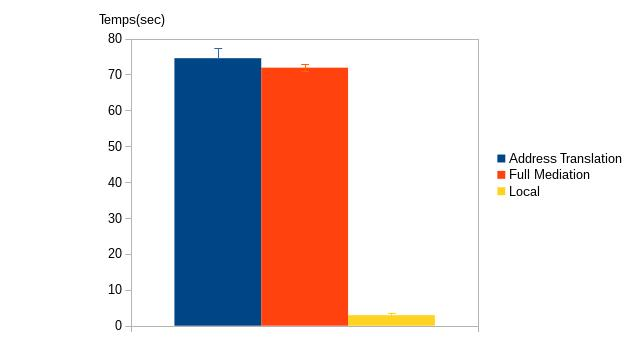
\includegraphics[scale=0.5]{mesures/graph/Littlemsg.jpg}
    \caption{Temps d'exécution de l'envoi d'un million de messages de 128o avec et sans Simterpose.}
    \label{Network_Little_Mediation}
\end{figure}

Lors de l'envoi de nombreux petits messages, on peut constater que la \textit{full mediation} est plus rapide que la \textit{médiation par traduction d'adresse} avec un écart moyen de 3 secondes. Lorqu'on utilise la \textit{médiation par traduction d'adresse} l'envoi de messages génère des appels systèmes et changements de contexte qui n'ont pas lieu en \textit{full mediation} puisque dans ce cas, comme nous l'avons expliqué en section \ref{paragraph:FULL_MEDIATION}, les appels systèmes ne sont pas exécutés. Ces derniers étant coûteux cela explique pourquoi la  \textit{médiation par traduction d'adresse} est moins rapide. De plus, en \textit{full mediation}, même si les appels systèmes sont bloqués, nous utilisons l'appel système \texttt{ptrace} pour effectuer nous-même les appels demandés par l'application que nous avons bloqués. Cette méthode même si elle reste moins coûteuse que l'exécution de l'appel système demandé consomme des cycles CPU, ce qui explique le faible écart entre les temps d'exécution moyen des deux types de médiation.

Lorsque l'on envoie un gros message, on constate que l'écart moyen entre les deux types de médiation est quasi nul, 0.03 secondes. Nous pensons que dans ce cas la \textit{médiation par traduction d'adresse} est légèrement plus rapide car nous envoyons un seul message de 1Mo de données. En effet, même si en \textit{full mediation} on a beaucoup moins de changement de contexte de par le blocage des appels systèmes ici on ne fait qu'un seul appel et la faible différence entre les deux médiations ne peut donc être dû à cela. Par contre, lors de l'envoi d'un tel message il faut prendre en compte la gestion de la mémoire car le message doit être stocké avant de pouvoir être envoyé par morceau sur le réseau. Ainsi, si on ne gère pas la mémoire de façon efficace on surconsomme des cycles CPU lorsqu'on accède à cette dernière. Or, nous n'avons pas encore mis en place de politique de gestion de mémoire particulière pour Simterpose. Néanmoins, si on regarde la largueur des intervalles des temps d'exécution, en \textit{médiation par traduction d'adresse} les temps d'exécution varient bien plus qu'en \textit{full mediation}. On peut donc supposer qu'avec une politique de gestion mémoire aussi efficace que celle qui est utilisée par le système la \textit{full mediation} serait probablement plus rapide que la \textit{médiation par traduction d'adresse} comme dans l'expérience précédente.

Ces expériences nous ont permis de montrer que lors de l'envoi de nombreux messages il vaut mieux privilégier la \textit{full mediation}. Nous avons également pu voir que pour envoyer de gros messages, les deux médiations se valent. De plus, la faible durée d'exécution d'une expérience nous permet de considérer que l'\textit{overhead} dû à la mise en place de Simterpose est acceptable. Ainsi, nous pouvons dire que notre implémentation du réseau de communications permet de faire de la virtualisation légère à ce niveau. Nous allons maintenant voir si il en est de même en ce qui concerne la gestion du temps.
